\section{Background}
Consider a formal example of communication in which he/she asks "what is the height of mount Everest ?" and second question would probably "Where is it located ?" Here in second question the questionnaire didn't explicitly mentioned the Mt.Everest, how ever we can easily understand that the questionnaire is interested to know about the location of Mt. Everest. It shows that the answer of this second question is dependent on the first one as well. In machine learning, such problem is known as sequence problem and the conventional neural network such as artificial neural network (ANN), convolution neural network (CNN) etc. has hard time to solve such type of problem.  


The limitation of these neural network leads to the development of Recurrent Neural Network architecture. The Recurrent Neural Network (RNN) is a Deep Neural Network which can be consider as the extension of convolution neural network \cite{chung2014empirical} and theoretically they are capable of learning long sequence of data. Unfortunately, in practice, RNNs don’t seem to be able to learn them because the gradients tend to either vanish (most of the time) or
explode (rarely, but with severe effects). The problem was explored in depth by Hochreiter\cite{hochreiter} and Bengio, et al.\cite{Bengio_2013}


\begin{figure}[h]
	\centering
	\subfigure[Long short term memory]{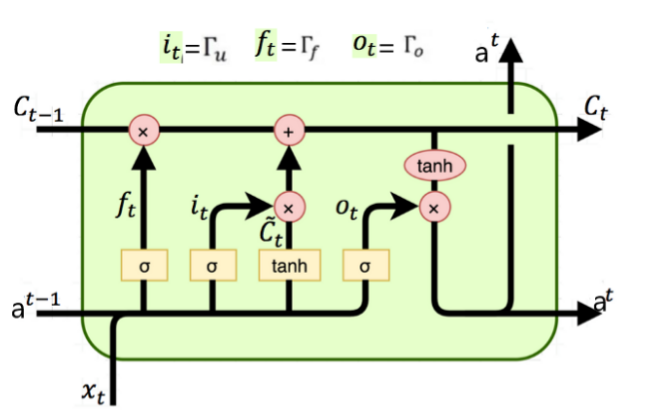
\includegraphics[width=0.5\textwidth]{Image-002.png}} 
	\subfigure[Gated recurrent unit ]{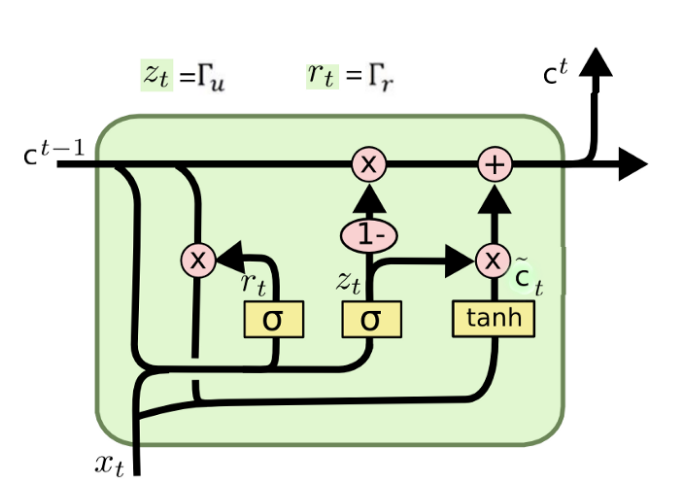
\includegraphics[width=0.5\textwidth]{Image-001.png}} 
	\caption{The general structure of recurrent	neural network models. (a) LSTM (b) GRU }
	\label{fig:foobar}
\end{figure}


\section{LSTM}
LSTM is a special kind of RNN capable of learning long-term dependencies introduced by Hochreiter et al. \cite{hochreiter}. LSTM model is explicitly designed to overcome the simple RNN long term dependency problem. This architecture consists of a forget gate, input gate and output gate. Forget is responsible for deciding what information are going to throw from cell state. It looks at $h_{t-1}$ and $x_t$, and outputs a number between 0 and 1 for each number in the cell state. The main operations in LSTM are formulated as \cite{shahi2020stock}:

Forget gate
\begin{equation}
	f_t = \sigma(w_f.[h_{t-1}, x_t]+b_f)
\end{equation}

\begin{equation}
	C_t = C_t \otimes {f_t}
\end{equation}

Input gate
\begin{equation}
	\bar{C_t}= tanh(W_i[h_{t-1}, x_t]+b_c)
\end{equation}

\begin{equation}
	i_t= \sigma(W_i[h_{t-1}, x_t]+b_i)
\end{equation}

\begin{equation}
	C_t= f_t \times C_{t-1} + i_t * \bar{C_t}
\end{equation}


Output gate
\begin{equation}
	o_t= \sigma(W_o[h_{t-1}, x_t]+b_o)
\end{equation}

\begin{equation}
	o_t= \sigma(W_o[h_{t-1}, x_t]+b_o)
\end{equation}
\begin{equation}
	h_t= o_t \times tanh(C_t)
\end{equation}
where $f_t$ is the value from the forget gate; b is the bias; $C_t$ is the value from the input gate; $i_t$ is the intermediate output.

\section{GRU}
GRU is a variation of LSTM architecture suggested by Cho et al. \cite{cho2014properties}. The main difference between LSTM and GRU architecture is that GRU merges the input and forget gates and converts them with an update gate, which reduces parameters in GRU as compare to the LSTM. It also merges cell state and hidden state and makes some other changes changes which makes  resulting model is simpler than standard LSTM models. The operation in GRU can be listed by following formulae \cite{shahi2020stock}:

\begin{equation}
	z_t =  \sigma(W_z.[h_{t-1}, x_t])
\end{equation}

\begin{equation}
	r_t =  \sigma(W_z.[h_{t-1}, x_t])
\end{equation}

\begin{equation}
	\bar{h_t} =  \tanh(W[r_t*h_{t-1}, x_t])
\end{equation}
\begin{equation}
	\bar{h_t} =  (1-z_t) * h_{t-1} + z_t * h_t
\end{equation}
	
where $z_t$ and $r_t$ are intermediate values obtained from the update and reset gates, respectively; $tanh$ is hyperbolic tangent function; $\sigma$ is the sigmoid function.

\section{Problem Statement}
Various studies has been conducted out to compare the performance of LSTM and GRU. In this study, Bitcoin price is predicted using two different models; one with LSTM cell and another with GRU cell, but with identical hyper-parameters in both.

\section{Objective}
The main objective of this study is to perform a normalized comparison on the performances of LSTM and GRU for bitcoin price prediction under the same conditions on metrics training time, MAE, RMSE, R$^2$ and DA.


